\documentclass{urticle}
\pgfplotsset{compat=1.13}

\begin{document}

	\begin{titlepage}
		
		
		
		\center % Center everything on the page
		
		
		
		%----------------------------------------------------------------------------------------
		%	HEADING SECTIONS
		%----------------------------------------------------------------------------------------
		
		\textsc{\LARGE Московский Физико-Технический Институт}\\[1,5cm] % Name of your university/college
		% Major heading such as course name
		\textsc{\Large Кафедра общей физики}\\[0.5cm]
		\textsc{\large Отчет о выполнении лабораторной работы \textnumero  2.1.1}\\[0.5cm] % Minor heading such as course title
		
		%----------------------------------------------------------------------------------------
		%	TITLE SECTION
		%----------------------------------------------------------------------------------------
		
		\HRule
		\\[0.4cm]
		{ \huge \bfseries Измерение удельной теплоёмкости воздуха при постоянном давлении}
		\\[0.2cm] % Title of your document
		\HRule
		\\[1.5cm]
		
		
		
		%----------------------------------------------------------------------------------------
		%	AUTHOR SECTION
		%----------------------------------------------------------------------------------------
		
		\begin{minipage}{0.7\textwidth}
			\begin{center} \large
				\emph{Автор:} Алексей \textsf{Домрачев} 615 группа
			\end{center}
		\end{minipage}
		\\[1.0cm]
		\begin{minipage}{0.9\textwidth}
			\begin{center} \large
				\emph{Преподаватель:} Александр Дмитриевич \textsf{Калашников} % Supervisor's Name
			\end{center}
		\end{minipage}
		\vfill 
	%	\begin{bottompar}
			
\includegraphics[width = 80 mm]{logo.png}	\\[1,0cm]
			{\large \today}
	%	\end{bottompar}
		% Fill the rest of the page with whitespace
		
	\end{titlepage}



\paragraph{Цель работы:}
	измерение повышения температуры воздуха в результате подвода тепла
		при стационарном течении через трубу
	и вычисление по результатам измерений теплоёмкости~$C_P$ воздуха
		при постоянном давлении.


\vspace{2\parskip}
\section{Постановка эксперимента}
\begin{wrapfigure}[10]{r}{.49\lw}
	\vspace{-6mm}
	\centering
	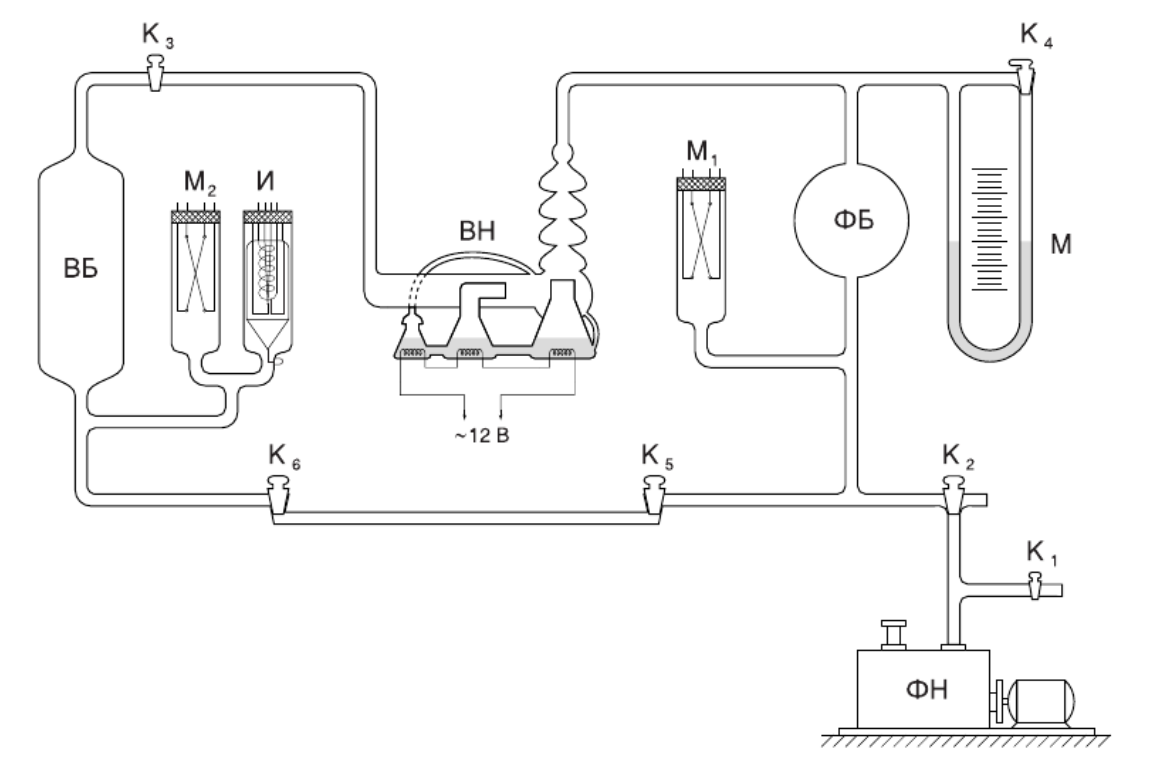
\includegraphics[width=.9\lw]{apparatus}
	\caption{Схема экспериментальной установки}
\end{wrapfigure}
Данная лабораторная работа предусматривает следующую методику измерений:
воздух продувается через калориметр, внутри которого установлен нагревательный элемент;
проводятся измерения мощности нагревателя~$W = IU$, объёмного расхода~$Q$ и изменения
температуры~$\Delta T$ потока воздуха.

\textbf{Обозначения:}\\[.5mm]
$K$~--- кран регулировки расхода;\\
ГС~--- газовый счётчик.

Нетрудно показать, что в ходе эксперимента \emph{вследствие стационарности процесса}
измеряется именно~$C_P$, причём
\begin{equation}
	C_P = \frac{\mu}{\rho}\frac{W - W'}{Q \Delta T},
\quad\text{где}~
	\rho \simeq \frac{\mu P}{RT},
\end{equation}
$W'$~--- мощность тепловых потерь. Логично предположить, что~$W' \simeq \beta \Delta T$,
тогда
\begin{equation}
\label{main-eq}
	\frac{W}{\Delta T} = \frac{\rho}{\mu} C_P \cdot Q + \beta.
\end{equation}
Из уравнения~(\ref{main-eq}) видно, что построение зависимости $\frac{W}{\Delta T}(Q)$
позволяет найти~$C_P$ и оценить долю теплопотерь
\begin{equation}
	\eta \equiv \frac{\mu\beta}{\rho C_P Q}.
\end{equation}


\section{Проведение измерений}
\paragraph{Начальные условия.} До начала и по окончании работы были записаны значения
температуры и давления в лаборатории, а также определена относительная влажность воздуха:
\vspace{-\parskip}
\begin{table}[h]\centering
\begin{tabular}{cccc}
\toprule
Время     & $t_0,~\CC$ & $P,~\hPa$&  $\chi,~\%$ \\
\midrule
14:00     &  22.6      &  987.7   &   70 \\
16:50     &  22.2      &  989.5   &   73 \\
\midrule
          &  22.4      &  988,6         \\
\bottomrule
\end{tabular}
\end{table}\\
По этим данным можно рассчитать плотность воздуха, которая в дальнейшем
будет полагаться постоянной:
\begin{equation}
	\rho = \frac{\mu P}{RT} = 1,17~\kg/\m^3.
\end{equation}

\paragraph{Прикидка.} При заданном расходе~$Q$ и известном сопротивлении
нагревательного элемента~$r = 35~\Ohm$ оценим силу тока~$I_0$, при протекании которого
температура потока увеличивается на~$\Delta T_0 = 1~\CC$:
\begin{equation}
	\frac{7}{2}R \approx \frac{\mu \cdot I_0^2 r}{\rho Q \Delta T_0}
\then
	I_0 = \sqrt{\frac{7R\rho \Delta T_0 \cdot Q}{2\mu r}} \simeq
	183~\m\A \cdot \sqrt{Q~[\l/\s]}.
\end{equation}
Величина сопротивления, измеренная непосредственно, составила
\begin{equation}
	r_e = \frac{5.275~\V}{151.68~\m\A} = 34.8~\Ohm.
\end{equation}

Следует отметить, что постоянная термопары~$\Xi = 42.3~\mk\V/\CC$, а значит,
для покрытия диапазона в~$9~\CC$ необходимо достигать значений термоЭДС
$\mathscr{E}_b \sim 380~\mk\V$.

При этом одному обороту стрелки газового счётчика соответствует объём прокачки $5~\l$.

\paragraph{Основные измерения.} Данные измерений при различных значениях~$Q_i$
приведены в таблице~\ref{opdata}, сведения о самих величинах~$Q_i$ сведены
в таблицу~\ref{rates}.


\begin{table}[h]
	\centering
	\begin{tabular}{cc|c}
\toprule
 $N,~\rev$ &  $\tau,~\s$ &  $Q_i,~\l/\s$ \\
\midrule
         3 &         165 &      0.090909 \\
         1 &         130 &      0.038462 \\
\bottomrule
\end{tabular}

	\caption{Объёмный расход воздуха\label{rates}}
\end{table}
\clearpage

\begin{table}[t]
	\renewcommand{\arraystretch}{.9}
	\centering
	\small
	\begin{tabular}{cccc|cccc}
\toprule
 $i$ &  $I,~\m\A$ &  $U,~\V$ &  $\mathscr{E},~\mk\V$ &   $W,~\m\W$ &  $\Delta T,~\CC$ &  $Q_i,~\l/\s$ &  $\frac{W}{\Delta T},~\m\W/\CC$ \\
\midrule
   1 &      77.17 &    2.682 &                    72 &   206.96994 &         1.702128 &      0.090909 &                      121.594840 \\
   1 &      99.83 &    3.470 &                   103 &   346.41010 &         2.434988 &      0.090909 &                      142.263565 \\
   1 &     123.14 &    4.282 &                   149 &   527.28548 &         3.522459 &      0.090909 &                      149.692455 \\
   1 &     141.25 &    4.914 &                   200 &   694.10250 &         4.728132 &      0.090909 &                      146.802679 \\
   1 &     160.09 &    5.571 &                   263 &   891.86139 &         6.217494 &      0.090909 &                      143.443866 \\
   1 &     177.02 &    6.163 &                   322 &  1090.97426 &         7.612293 &      0.090909 &                      143.317426 \\
   1 &     183.83 &    6.401 &                   354 &  1176.69583 &         8.368794 &      0.090909 &                      140.605180 \\
   2 &      49.23 &    1.714 &                    52 &    84.38022 &         1.229314 &      0.038462 &                       68.640064 \\
   2 &      80.01 &    2.788 &                   126 &   223.06788 &         2.978723 &      0.038462 &                       74.887074 \\
   2 &      99.19 &    3.457 &                   192 &   342.89983 &         4.539007 &      0.038462 &                       75.545119 \\
   2 &     112.75 &    3.931 &                   253 &   443.22025 &         5.981087 &      0.038462 &                       74.103623 \\
   2 &     124.49 &    4.342 &                   322 &   540.53558 &         7.612293 &      0.038462 &                       71.008245 \\
   2 &     131.72 &    4.594 &                   364 &   605.12168 &         8.605201 &      0.038462 &                       70.320459 \\
   2 &     138.06 &    4.817 &                   412 &   665.03502 &         9.739953 &      0.038462 &                       68.279081 \\
\bottomrule
\end{tabular}

	\caption{Основные данные измерений и расчёты\label{opdata}}
\end{table}

\begin{figure}[t]
\centering
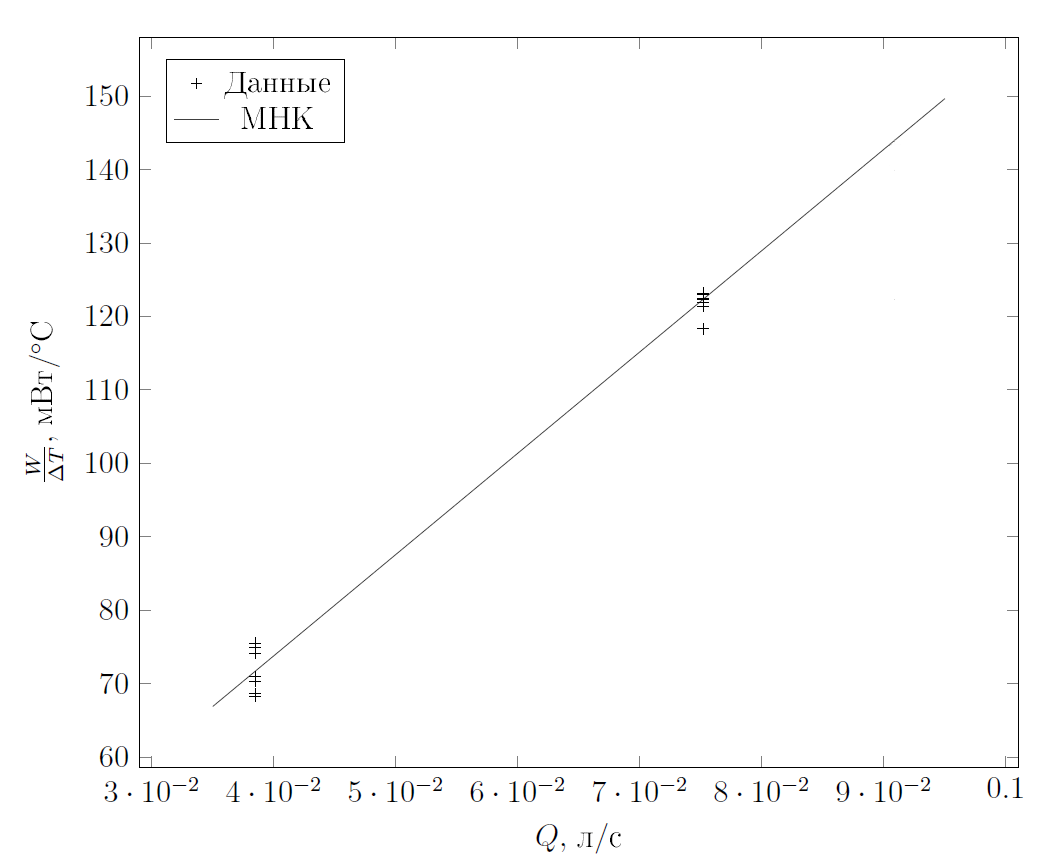
\includegraphics[width = 150 mm]{graph1.png}	\\[1,0cm]
\caption{График зависимости $\dfrac{W}{\Delta T}$ от $Q$ \label{plot}}
\end{figure}
\clearpage


\section{Итоги}
Обрабатывая точки исследуемой зависимости по МНК,
получаем значения коэффициентов зависимости~(\ref{main-eq}):
\begin{gather}
	\frac{\rho}{\mu}C_P = (1.38 \pm 0.03)~\k\J/(\K \cdot \m^3)
\Longrightarrow\\
	C_P = (33.6 \pm 0.6)~\J/(\mol \cdot \K) = \boxed{(4.0 \pm 0.1) R;}
\\[2\parskip]
	\beta \approx 20~\m\W/\K
\then
	\eta \sim (15 \div 40)\,\%.
\end{gather}

\paragraph{Комментарий.} Полученная в результате выполнения настоящей лабораторной работы зависимость имеет <<хороший>>, линейный вид ($\mathfrak{R} = 0.9965$), однако итоговое
значение~$C_P$ завышено на~$15\,\%$ по сравнению с теоретическим, что на порядок превышает
оценку погрешности косвенного измерения.

%\textsl{Поскольку такой же результат был получен в ходе обработки моим коллегой,
%выполнявшим эту работу вместе со мной, смею предположить, что величины,
%заданные в описании лабораторной работы, имеют в действительности отличные
%от указанных значения.}

\end{document}
